% %%%%%%%%%%%%%%%%%%%%%%%%%%%%%%%%%%%%%%%%%%%%%%%%%%%%%%%%%%%%%%%%%%%%%%%%%%%%%
% %%%%%%%%%%%%%%%%%%%%%%%%%%%%%%%%%%%%%%%%%%%%%%%%%%%%%%% Building on Mann 1995
% %%%%%%%%%%%%%%%%%%%%%%%%%%%%%%%%%%%%%%%%%%%%%%%%%%%%%%%%%%%%%%%%%%%%%%%%%%%%%

\chapter{Finite Poloidal Lifetimes}
\label{ch_lifetimes}

This is why we do 2.5D... you can't resolve these effects in a 3D model. It's too expensive. 

\todo{Do we see a difference between \vec{k} (momentum) and the group velocity? Poynting flux will always be pretty much along the field line, since $B_3$ is small and $E_3$ is zero, but the wave vector need not be. This is a question of coupling/converting to compressional waves, I guess. }

\todo{Look at McKenzie and Westphal. Waves incident on the bow shock, etc, at weird angles. }

\todo{Look at the E to B ratio. Compare to the \Alfven speed and to the height-integrated Pedersen conductivity. }

% =============================================================================
% =============================================================================
% =============================================================================
\section{Finite Poloidal Lifetimes}

Radoski 1974 \cite{radoski_1974}. Ding 1995\cite{ding_1995}. Mann 1995\cite{mann_1995}. 

\todo{Look at Mann's poloidal lifetime, $\dd{\omega_A'} \lambda$ where $\lambda \sim \frac{\azm}{2 \pi r}$. }

\begin{figure}[H]
    \centering
    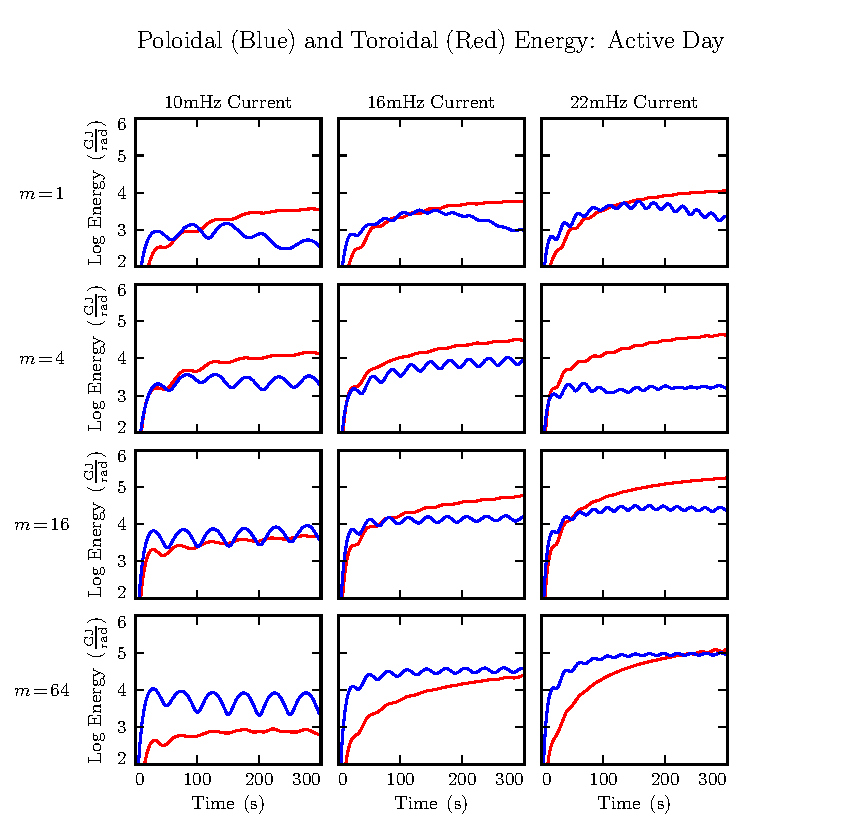
\includegraphics[width=\textwidth]{figures/UP_UT_J_1.pdf}
    \caption[Current-Driven Poloidal and Toroidal Energy: Active Day]{}
    \label{fig_UP_UT_J_1}
\end{figure}

\begin{figure}[H]
    \centering
    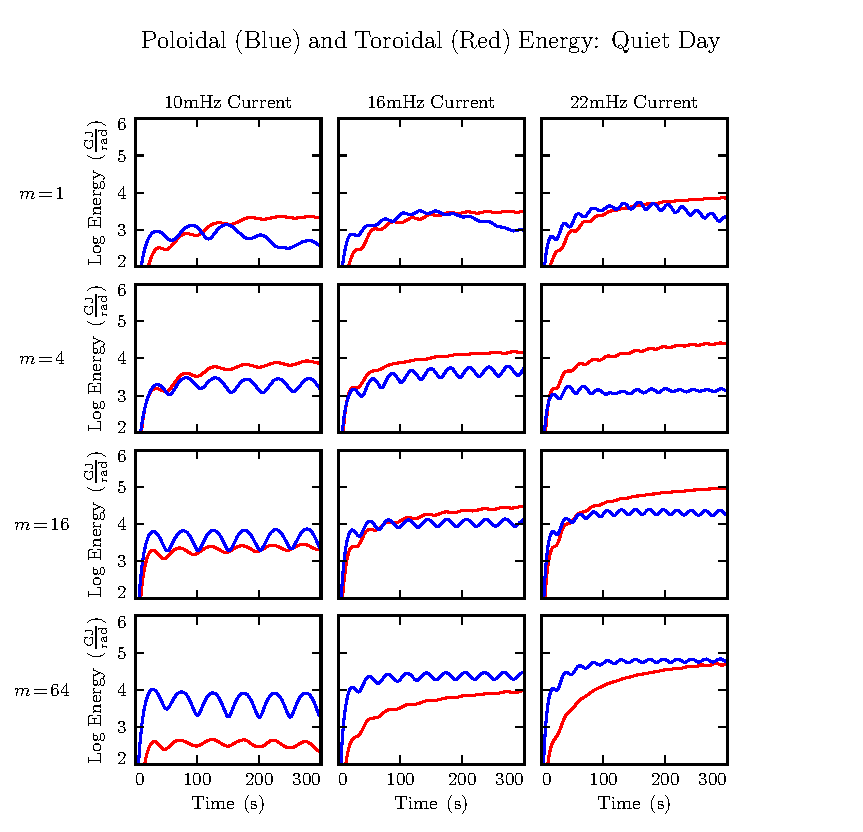
\includegraphics[width=\textwidth]{figures/UP_UT_J_2.pdf}
    \caption[Current-Driven Poloidal and Toroidal Energy: Quiet Day]{}
    \label{fig_UP_UT_J_2}
\end{figure}

\begin{figure}[H]
    \centering
    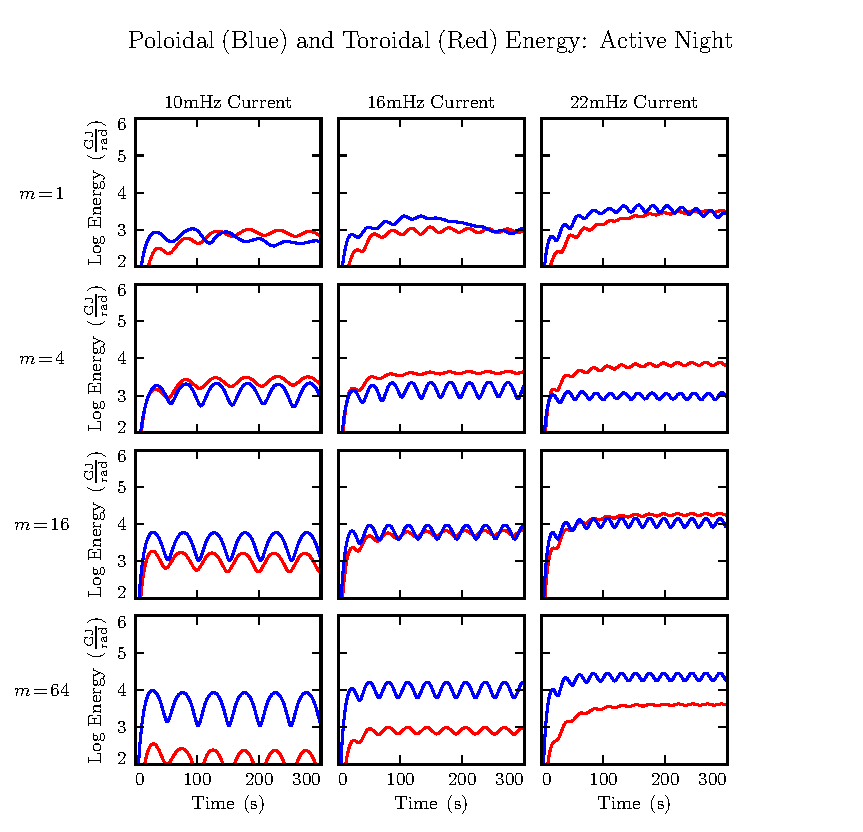
\includegraphics[width=\textwidth]{figures/UP_UT_J_3.pdf}
    \caption[Current-Driven Poloidal and Toroidal Energy: Active Night]{}
    \label{fig_UP_UT_J_3}
\end{figure}

\begin{figure}[H]
    \centering
    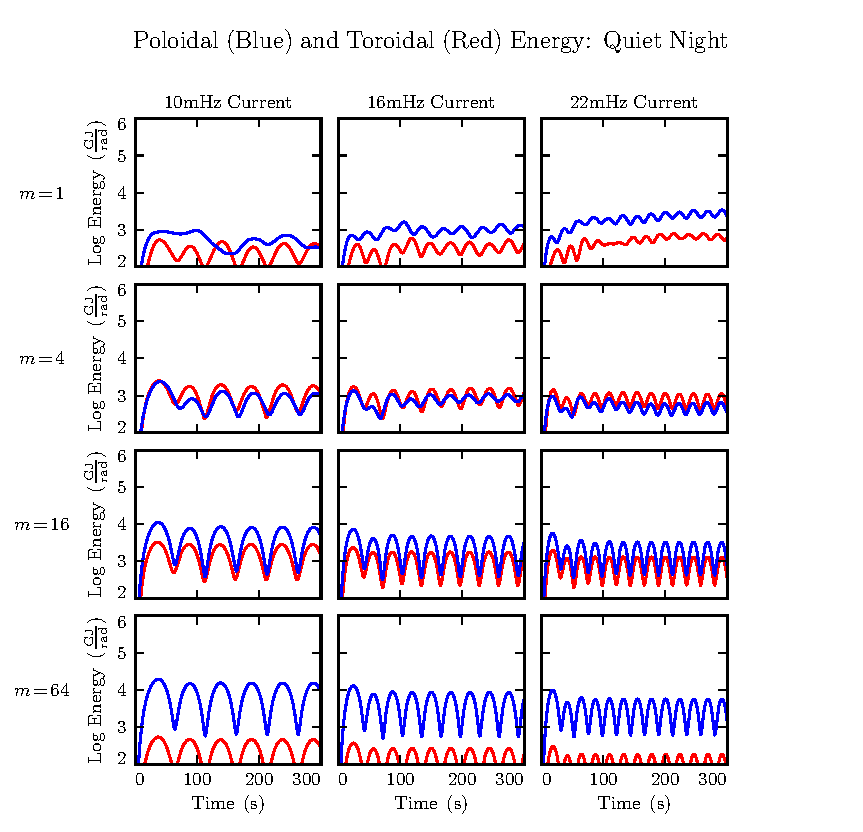
\includegraphics[width=\textwidth]{figures/UP_UT_J_4.pdf}
    \caption[Current-Driven Poloidal and Toroidal Energy: Quiet Night]{}
    \label{fig_UP_UT_J_4}
\end{figure}

% =============================================================================
% =============================================================================
% =============================================================================
\section{Development of Fine Structure}

\todo{These plots are very pretty, but it's not clear that they do a good job of communicating the important information. }

\begin{figure}[H]
    \centering
    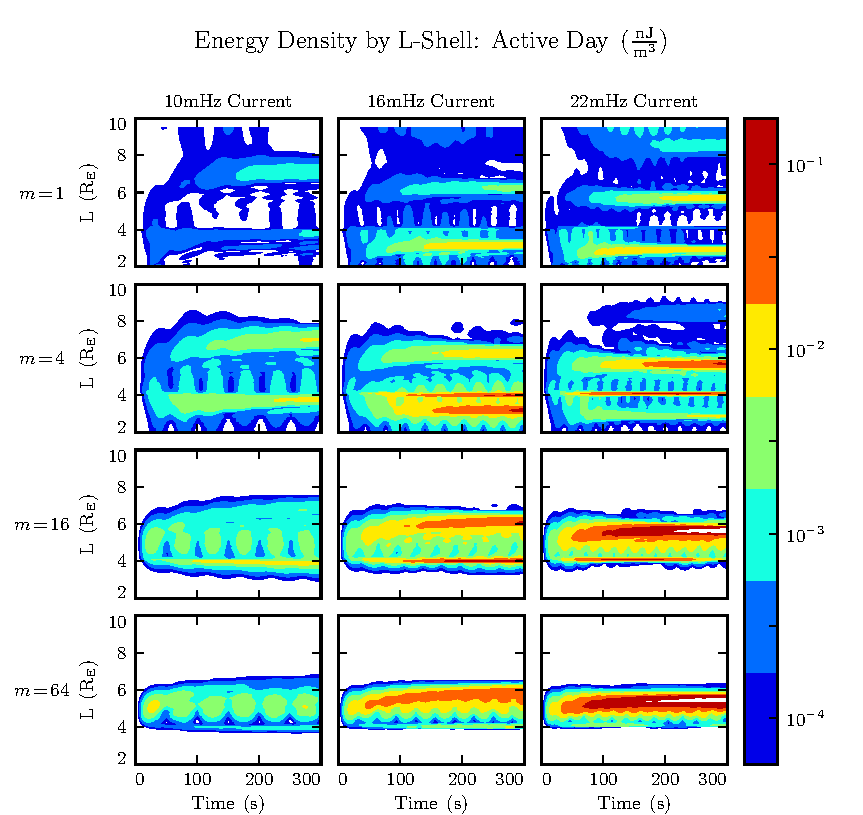
\includegraphics[width=\textwidth]{figures/ulayers_J_1.pdf}
    \caption[Energy Density by L-Shell: Active Day]{}
    \label{fig_ulayers_J_1}
\end{figure}

\begin{figure}[H]
    \centering
    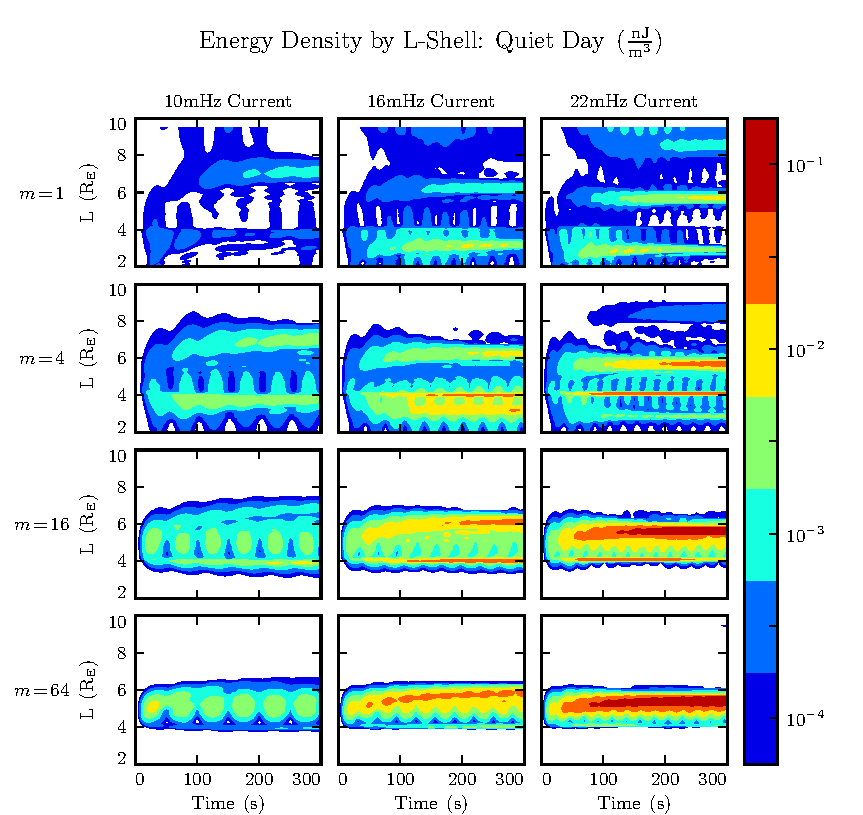
\includegraphics[width=\textwidth]{figures/ulayers_J_2.pdf}
    \caption[Energy Density by L-Shell: Quiet Day]{}
    \label{fig_ulayers_J_2}
\end{figure}

\begin{figure}[H]
    \centering
    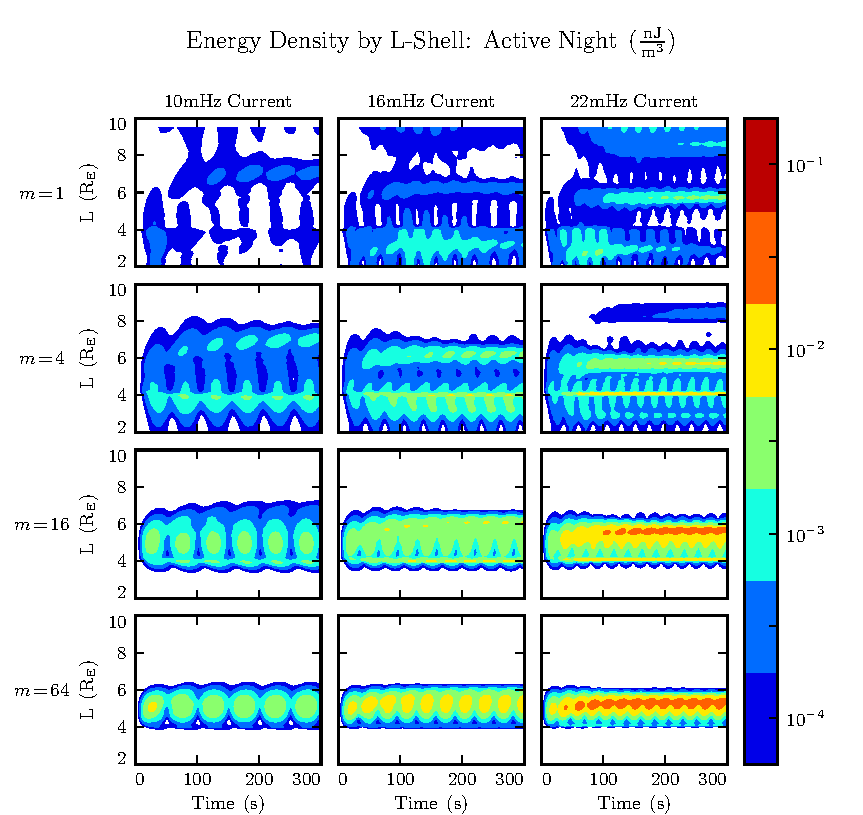
\includegraphics[width=\textwidth]{figures/ulayers_J_3.pdf}
    \caption[Energy Density by L-Shell: Active Night]{}
    \label{fig_ulayers_J_3}
\end{figure}

\begin{figure}[H]
    \centering
    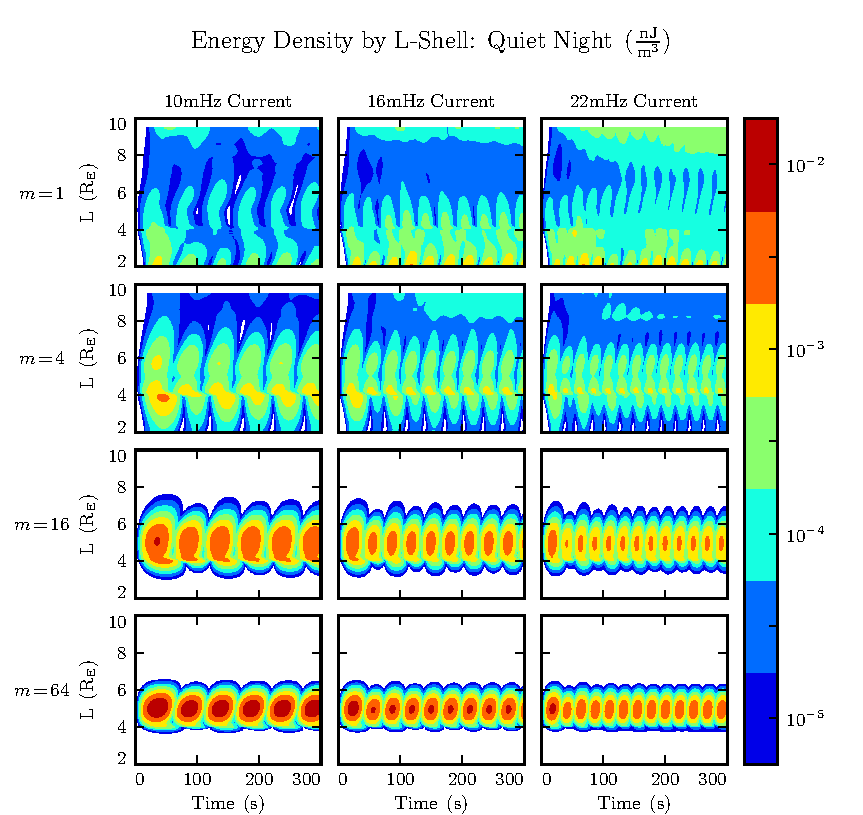
\includegraphics[width=\textwidth]{figures/ulayers_J_4.pdf}
    \caption[Energy Density by L-Shell: Quiet Night]{}
    \label{fig_ulayers_J_4}
\end{figure}







